\chapter{Experimental Setup}
\section{Equipment}
\subsection{ESC Assessment}
The most important component for the analysis in this project is the ESC. Therefore, a thorough assessment of different ESCs and their firmware was made. The criteria to pick the particular board took into account that it is to be used with the Voliro OMAV at the ASL in t ETH Zurich depicted in Figure \ref{fig: mav_photo}. The parameters accounted for as well as the top rated ESCs are shown in Table \ref{tab:tab_escs}. Further analyzed ESCs are show in Appendix \ref{sec:appendix_escs}.

\begin{table}
\small
% \addtolength{\leftskip} {-2cm}
%\addtolength{\rightskip}{-2cm}

\begin{center}
 	\caption{ESC protocols' speeds}\vspace{1ex}
 	\label{tab:tab_escs}
\makebox[\textwidth]{
	 \begin{tabular}{l|rrrrrrrrr}
	 \hline
	ESC Model & Speed feedback & Brake  & Size [mm] & Motors & Protocol & Current Sens & Firmware & Efficiency\\ \hline \hline
	
	Flycolor X-Cross 4in1		&	Telemetry	&	Yes &	42x45x7.5	&	4	&	Dshot	&	Telemetry	&	BlHeli\_32	& 	Sine Mod\\
	Lumenier Elite 4in1			&	Telemetry	&	Yes &	43x46x7.5	&	4	&	Dshot	&	Telemetry	&	BlHeli\_32	&	Sine Mod\\
	Holybro Tekko32 F3 Metal	&	Telemetry	&	Yes	&	42x42x4		&	4	&	Dshot	&	Analog		&	BlHeli\_32	&	Sine Mod\\
	Myxa by Zubax				&	UAVCAN		&	Yes	&	57x38x24	&	1	&	UAVCAN	&	UAVCAN		&	Sapog v2	&	FOC\\
	Holybro Koleta20			&	UAVCAN		&	Yes	&	40x27x5		&	1	&	UAVCAN	&	UAVCAN		&	Sapog v2	&	FOC\\
	\end{tabular}
}

\end{center}
\footnotesize{NOTE: All ESCs that support Dshot in this table support all analog protocols and Bidirectional Dshot}
\end{table}

Therefore, we can see that there are two trends of high-performance ESCs. The first one relates to the most modern ESCs used in drone racing. They are very similar since they are mostly manufactured to use the BlHeli\_32 firmware. This firmware, allows for multiple parameter modification via the software BlHeliSuite (see Appendix \ref{sec:firm_blheli} for instructions). Given their modularity, they can be made into very small boards. For instance, they now come in 4 in 1 boards (i.e. one board includes 4 ESCs). The other group of high-performing ESCs use UAVCAN as communication protocol with the FC. This gives the advantage of less cabling. They use FOC which makes them more efficient than Sine Modulation versions specially at low rotor speed (below 1000 RPM). These also have possibility of on-board speed control, but it does not include any feed-forward prior.  The Holybro Tekko32 F3 ESC was then selected for investigation due to the wide variety of protocols it supports, it's multiple rotor support, good heat-sinking and flexibility to change parameters. Please refer to Section \ref{sec: esc_dig_prot} for a more thorough description of Dshot, Bidirectional Dshot and UAVCAN protocols.

\subsection{Overall setup}

The rig shown in Figure \ref{fig:exp_setup} was setup for testing purposes. The two propellers are positioned one in front of each other at 11.48cm separation, they are spun in opposite directions and positioned to exert thrust in the same direction. All of this, to emulate the behavior of rotor pairs in each arm of the OMAV presented in the introduction. The core components of this setup are as follows:
\begin{itemize}
	\item 2 BLDC motors by KDE Direct model 2315XF-885Kv 14 poles.
	\item 1 clockwise Hobbyking Propeller 9in diameter 4.7in pitch.
	\item 1 counter-clockwise Hobbyking Propeller 9in diameter 4.7in pitch.
	\item 1 Tekko32 F3 Metal ESC.
	\item $1\mu F$ capacitor.
	\item 1 6S LiPo battery.
	\item Pixhawk 4 flight controller
	\item Laptop (running Ubuntu 18.04 for firmware compilation).
	\item Support towers to attach motors.
\end{itemize}

\begin{figure} 
    \centering
    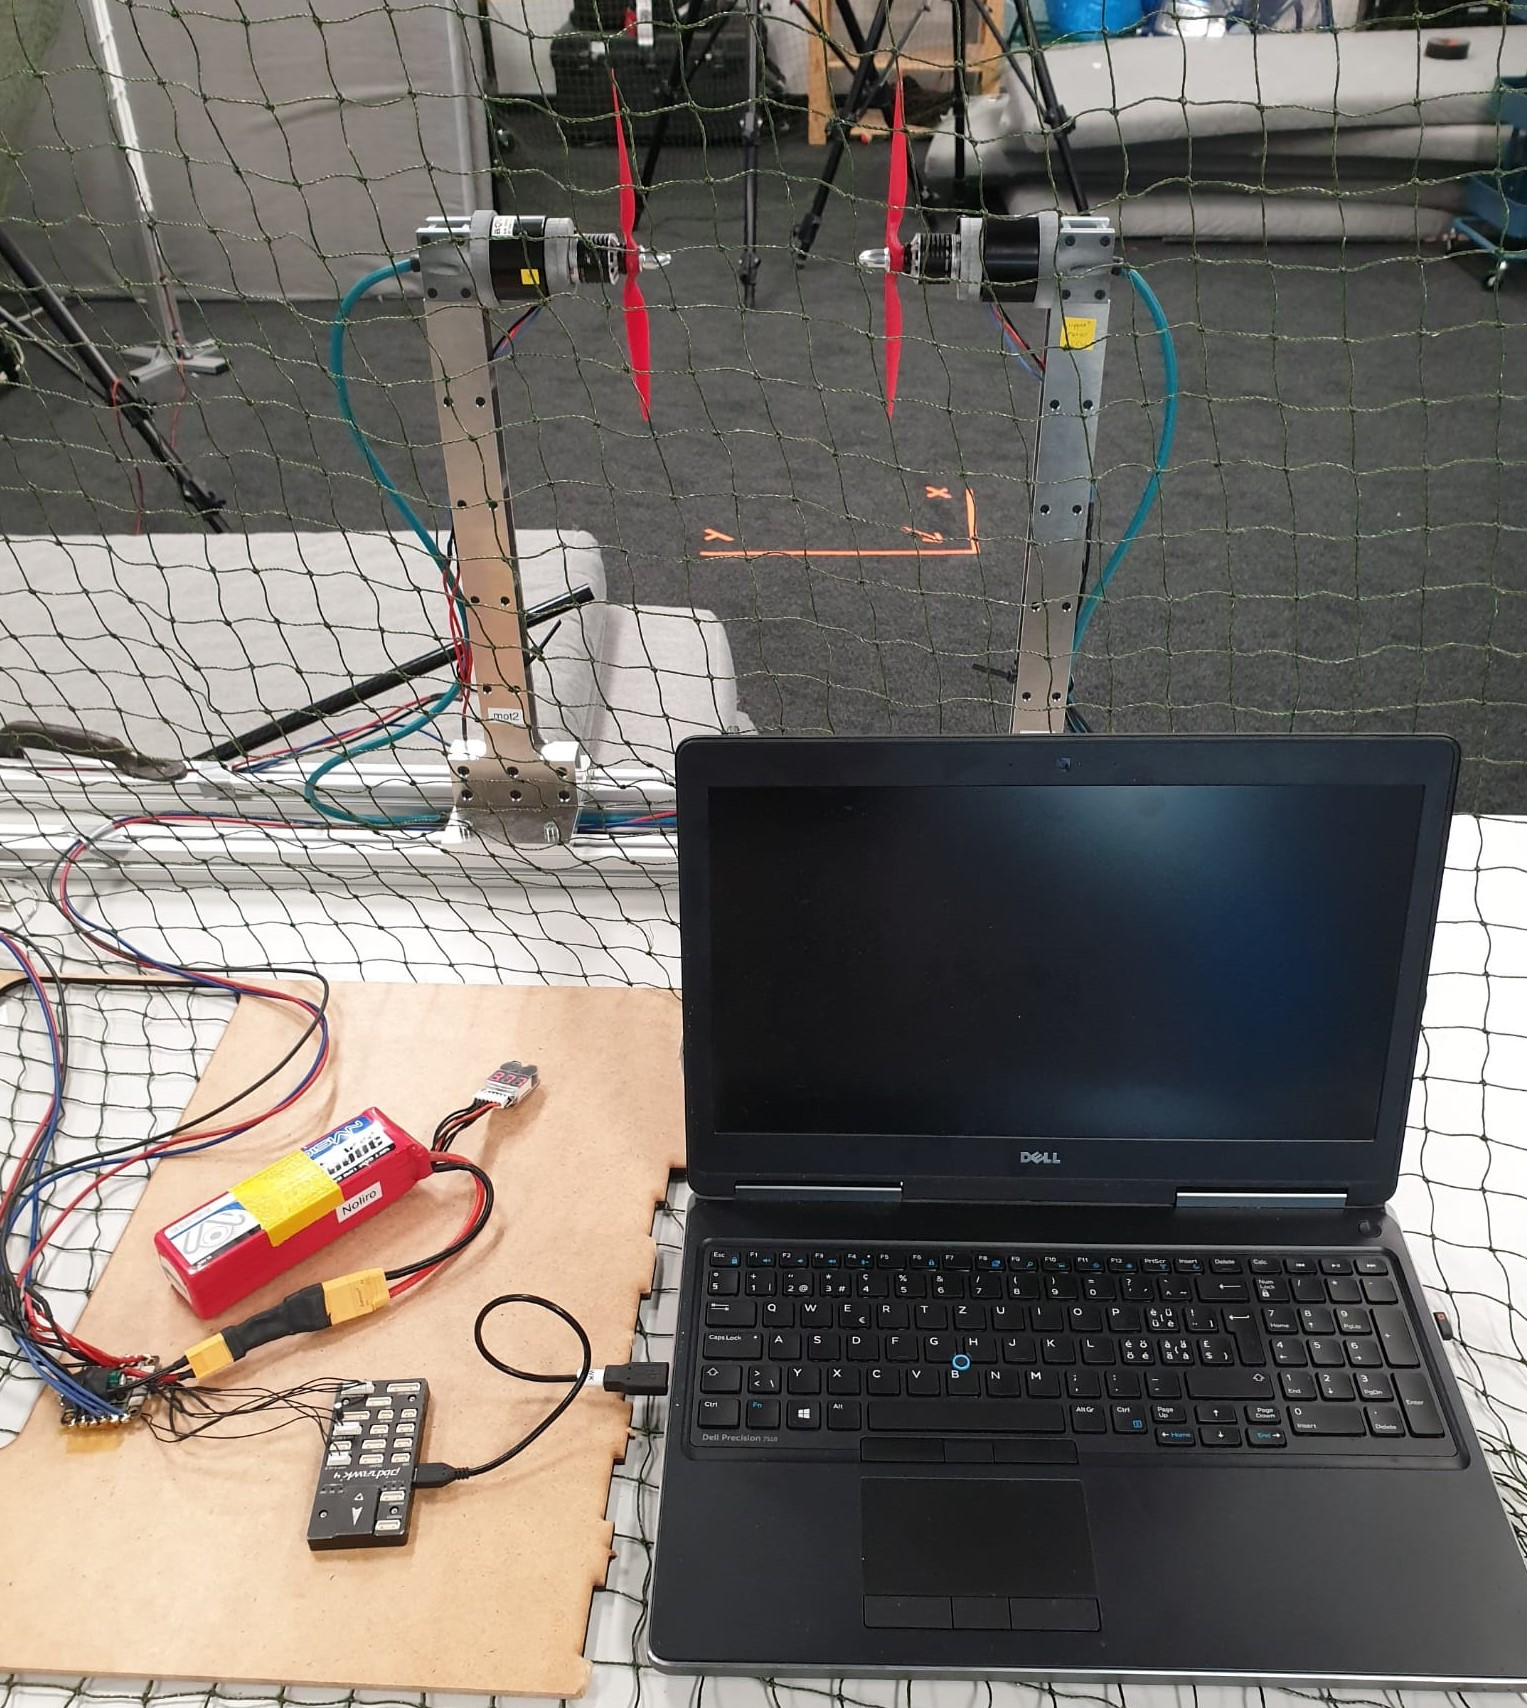
\includegraphics[width=0.9\textwidth]{images/setup_photo.png}
    \caption{Experimental setup}
    \label{fig:exp_setup}
\end{figure}


\subsection{Electrical Wiring}
Given the non-ambiguous nature of the Dshot protocol wiring, it is important to show how it should be done correctly. Hence, Figure \ref{fig:esc_wiring} show this setup in more detail.
\newline
Note that it is crucial to have the decoupling capacitor across the Analog to Digital Converter (ADC) of the Pixhawk. The reason to have it is to filter the noise induced by high frequency Dshot signals (on yellow). In fact, with no filtering, the ADC line is mostly composed of noise. A value of $0.1\mu F$ showed to attenuate this noise more than enough. It is also key to use ADC1\_SPARE\_1 (not ADC1\_SPARE\_2) as it has a lower reference voltage of 3.3V against 6.6V, which leads to higher resolution.
\newline
It is also important to mention that the ground wire can be connected to the ground pin in any port (usually the last pin). Further details on wiring can be seen in Appendix \ref{sec:px4_instructions}

\begin{figure} 
    \centering
    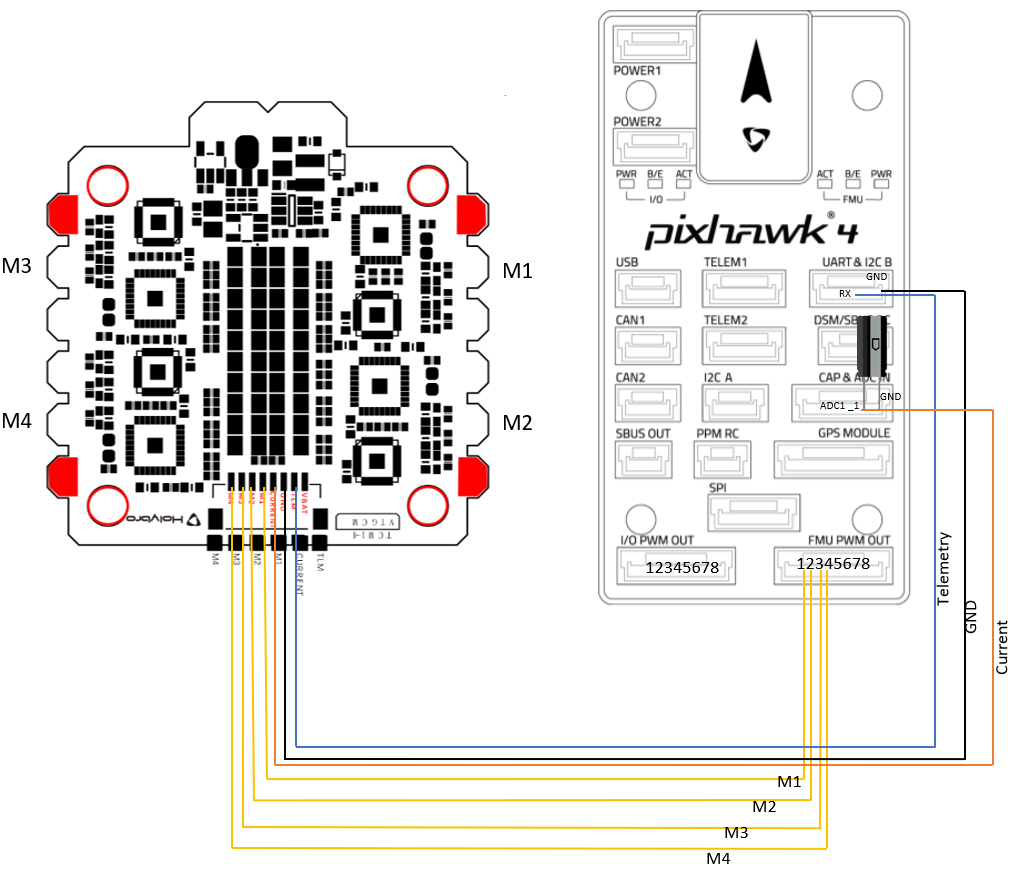
\includegraphics[width=0.9\textwidth]{images/esc_wiring.png}
    \caption{ESC-FC wiring. \textit{Left: ESC}, \textit{Right:} FC}
    \label{fig:esc_wiring}
\end{figure}

\section{Software toolboxes}
As developing tools for testing and firmware configuration, three pieces of software were used.
\newline

\textit{PX4} is the firmware running on the flight controller. It provides an on-board operating system called NuttX used in the Pixhawk 4. Additionally, it provides with a publisher-subscriber framework called \textit{uORB} on top of which this investigation constructed. There are four structures of interest in the PX4 firmware for this purpose: drivers, modules, mixers and messages. A module is a piece of code with a specific functionality that usually runs in parallel to other modules. Drivers are special kinds of modules whose whole purpose is to interface the high-level of abstraction module structure with the low level embedded software used to generate physical signals to drive actuators. Mixers are used to normalize and transform input or output control signals. For example there are mixers that translate desired angular position into thrust values in each motor. Lastly, messages define the structure of the information sent via uORB.
\newline

\textit{QGroundControl} is the Ground station software platform used with PX4. In general it allows to deploy full drones to different types of missions. It also 
\newline

\textit{BlHeliSuite} is the main software used to update the firmware of ESCs running with BlHeli\_32. It not only allows to download newer versions, but also let's change parameters of the ESC behavior. These include:

\begin{itemize}
	\item Rump-up power: Limits power on startup and low RPM.
	\item Motor timing: determines when angular positions with respect to magnetic poles when commutation happen. Beneficial to change with high inductance motors.
	\item PWM frequency: Modulation frequency to switch MOSFETs.
	\item Demag compensation: detects and compensates for high inductance motors.
	\item Sine Modulation: Approximation to FOC control.
	\item Maximum acceleration.
	\item Motor Direction.
	\item Brake on stop. Applies regenerative brake.
\end{itemize}

\textit{Ardupilot} is another flight controller firmware such as PX4. This was only used as an interface to configure ESCs using BlHeliSuite. Instructions on how to use it to configure BlHeli\_32 are detailed in Appendix \ref{sec:firm_blheli}
\newline

\section{Software developed}
The main aim of software development during this project was to drive motors using the Dshot protocol and obtain the telemetry packet to analyze responses and the feasibility of feedback control.

\subsection{Existent software}
The software developed for this project was built on top of PX4 v1.10. The components of interest from PX4 are described below.
\newline

\textit{Dshot driver: } This version of PX4 is the only one that provides support for Dshot. The driver is called "dshot.cpp". It runs the main control thread that receives commands, checks for updates and publishes received telemetry packets to uORB.
\newline

\textit{Telemetry: } "telemetry.cpp". There is a telemetry handler that receives the serial stream and decodes it in the appropriate format. Since the data from all motors is shared through same telemetry line, they have to be multiplexed. This handler performs the multiplexing in a blocking manner for up to 25ms if no message is received.
\newline

\subsection{Elements added/modified}
\textit{Mixer: } "quad\_x\_v2.main". This mixer provides pass-through mixing, that is, it takes a control command and directly passes it as a percentage throttle to be commanded to the ESC. Furthermore, in order to be loaded, it needs to be assigned to an airframe that itself is called on start-up within the PX4 framework. To do so, the "4001\_quad\_x" airframe was modified to pick the new mixer.
\newline

\textit{Dshot controller: } "dshot\_controller.cpp". This is the core of the functionalities developed during this project.  It publishes to the "actuator\_controls\_0" topic at 400Hz, derived from the "vehicular\_angular\_velocity" topic. Furthermore, it provides with user interaction through the Nutshell. The allowed commands are:
\begin{itemize}
	\item static throttle command to any of the 4 motors or all with non-blocking behavior.
	\item Sinusoidal wave of desired amplitude and period.Period can be changed from 10ms to 10000ms.
	\item Random waveform at a certain offset.
	\item Sinusoidal sweep (chirp) signal.
\end{itemize}
A thorough explanation of how setup and utilize this tool is found in Appendix \ref{sec:px4_instructions}.